\documentclass[a4paper,11.5pt]{article}
\usepackage[textwidth=170mm, textheight=230mm, inner=20mm, top=20mm, bottom=30mm]{geometry}
\usepackage[normalem]{ulem}
\usepackage[utf8]{inputenc}
\usepackage[T1]{fontenc}
\PassOptionsToPackage{defaults=hu-min}{magyar.ldf}
\usepackage{pgfplots}
\pgfplotsset{compat=1.10}
\usepgfplotslibrary{fillbetween}
\usepackage[magyar]{babel}
\usepackage{amsmath, amsthm,amssymb,paralist,array, ellipsis, graphicx, float, bigints,tikz}
%\usepackage{marvosym}

\makeatletter
\renewcommand*{\mathellipsis}{%
	\mathinner{%
		\kern\ellipsisbeforegap%
		{\ldotp}\kern\ellipsisgap
		{\ldotp}\kern\ellipsisgap%
		{\ldotp}\kern\ellipsisaftergap%
	}%
}
\renewcommand*{\dotsb@}{%
	\mathinner{%
		\kern\ellipsisbeforegap%
		{\cdotp}\kern\ellipsisgap%
		{\cdotp}\kern\ellipsisgap%
		{\cdotp}\kern\ellipsisaftergap%
	}%
}
\renewcommand*{\@cdots}{%
	\mathinner{%
		\kern\ellipsisbeforegap%
		{\cdotp}\kern\ellipsisgap%
		{\cdotp}\kern\ellipsisgap%
		{\cdotp}\kern\ellipsisaftergap%
	}%
}
\renewcommand*{\ellipsis@default}{%
	\ellipsis@before
	\kern\ellipsisbeforegap
	.\kern\ellipsisgap
	.\kern\ellipsisgap
	.\kern\ellipsisgap
	\ellipsis@after\relax}
\renewcommand*{\ellipsis@centered}{%
	\ellipsis@before
	\kern\ellipsisbeforegap
	.\kern\ellipsisgap
	.\kern\ellipsisgap
	.\kern\ellipsisaftergap
	\ellipsis@after\relax}
\AtBeginDocument{%
	\DeclareRobustCommand*{\dots}{%
		\ifmmode\@xp\mdots@\else\@xp\textellipsis\fi}}
\def\ellipsisgap{.1em}
\def\ellipsisbeforegap{.05em}
\def\ellipsisaftergap{.05em}
\makeatother

\usepackage{hyperref}
\hypersetup{
	colorlinks = true	
}

\DeclareMathOperator{\Int}{int}
\DeclareMathOperator{\tg}{tg}
\DeclareMathOperator{\ctg}{ctg}
\DeclareMathOperator{\Th}{th}
\DeclareMathOperator{\sh}{sh}
\DeclareMathOperator{\ch}{ch}
\DeclareMathOperator{\arsh}{arsh}
\DeclareMathOperator{\arch}{arch}
\DeclareMathOperator{\arth}{arth}
\DeclareMathOperator{\arcth}{arcth}
\DeclareMathOperator{\grad}{grad}
\DeclareMathOperator{\arc}{arc}
\DeclareMathOperator{\arctg}{arc tg}
\DeclareMathOperator{\arcctg}{arc ctg}
\newcommand{\norm}[1]{\left\lVert#1\right\rVert}

\begin{document}
	%%%%%%%%%%%RÖVIDÍTÉSEK%%%%%%%%%%
	\setlength\parindent{0pt}
	\def\a{\textbf{a}}
	\def\b{\textbf{b}}
	\def\N{\hskip 10 true mm}
	\def\a{\textbf{a}}
	\def\b{\textbf{b}}
	\def\c{\textbf{c}}
	\def\d{\textbf{d}}
	\def\e{\textbf{e}}
	\def\gg{$\gamma$}
	\def\vi{\textbf{i}}
	\def\jj{\textbf{j}}
	\def\kk{\textbf{k}}
	\def\fh{\overrightarrow}
	\def\l{\lambda}
	\def\m{\mu}
	\def\v{\textbf{v}}
	\def\0{\textbf{0}}
	\def\s{\hspace{0.2mm}\vphantom{\beta}}
	\def\Z{\mathbb{Z}}
	\def\Q{\mathbb{Q}}
	\def\R{\mathbb{R}}
	\def\C{\mathbb{C}}
	\def\N{\mathbb{N}}
	\def\Rn{\mathbb{R}^{n}}
	\def\Ra{\overline{\mathbb{R}}}
	\def\sume{\displaystyle\sum_{n=1}^{+\infty}}
	\def\sumn{\displaystyle\sum_{n=0}^{+\infty}}
	\def\biz{\emph{Bizonyítás:\ }}
	\def\narrow{\underset{n\rightarrow+\infty}{\longrightarrow}}
	\def\limn{\displaystyle\lim_{n\to +\infty}}
	%	\def\definition{\textbf{Definíció:\ }}
	%	\def\theorem{\textbf{Tétel:\ }}
	%\def\note{\emph{Megjegyzés:\ }}
	%\def\example{\textbf{Példa:\ }} 
	
	\theoremstyle{definition}
	\newtheorem{theorem}{Tétel}[subsubsection] % reset theorem numbering for each chapter
	
	\theoremstyle{definition}
	\newtheorem{definition}[theorem]{Definíció} % definition numbers are dependent on theorem numbers
	\newtheorem{example}[theorem]{Példa} % same for example numbers
	\newtheorem{exercise}[theorem]{Házi feladat} % same for example numbers
	\newtheorem{note}[theorem]{Megjegyzés} % same for example numbers
	\newtheorem{task}[theorem]{Feladat} % same for example numbers
	\newtheorem{revision}[theorem]{Emlékeztető} % same for example numbers
	%%%%%%%%%%%%%%%%%%%%%%%%%%%%%%%%%
	\begin{center}
		{\LARGE\textbf{Analízis 3. A szakirány}}
		\smallskip
		
		{\Large Gyakorlati jegyzet}
		
		\smallskip
		9. óra.
	\end{center}
	A jegyzetet \textsc{Umann} Kristóf készítette \textsc{Filipp} Zoltán István gyakorlatán.\\ (2017. április 20.
	
\includegraphics[height=3cm]{kepek/420.jpg}) %TODO 420!!!
	\subsection{Irány menti és parciális derivált}
	\begin{revision}
		\begin{enumerate} 
			\item $f\in\R{^n}\to\R;\quad 1\leq n\in\N;\quad a\in\int\mathcal{D}_f;\quad e\in\R^n;\quad \norm{e}_{\R^n}=1 m\quad F(t):=f(a+te),\quad t\in k_\delta(0)\quad (\delta$ alkalmas $a+te\in\mathcal{D}_f).$ Ha
			\[ \exists F'(0):=\delta_ef(a)\in\R \]
		\end{enumerate}
	\end{revision}
	\begin{task}
		\[ f(x,y):=x^2-xy+y^2\quad ((x,y)\in\R^2) \]
		Legyen továbbá $e$ az $x$ tengellyel 60 fokos szöget bezáró egységvektor.
		Ekkor:
		\begin{enumerate}
			\item $\delta_{e}f(1,1)=?$
			\item Milyen $e$ mentén lesz $\delta_{e}f(1,1)$ min ill. max?
		\end{enumerate}
		\begin{figure}[H]
			\centering
			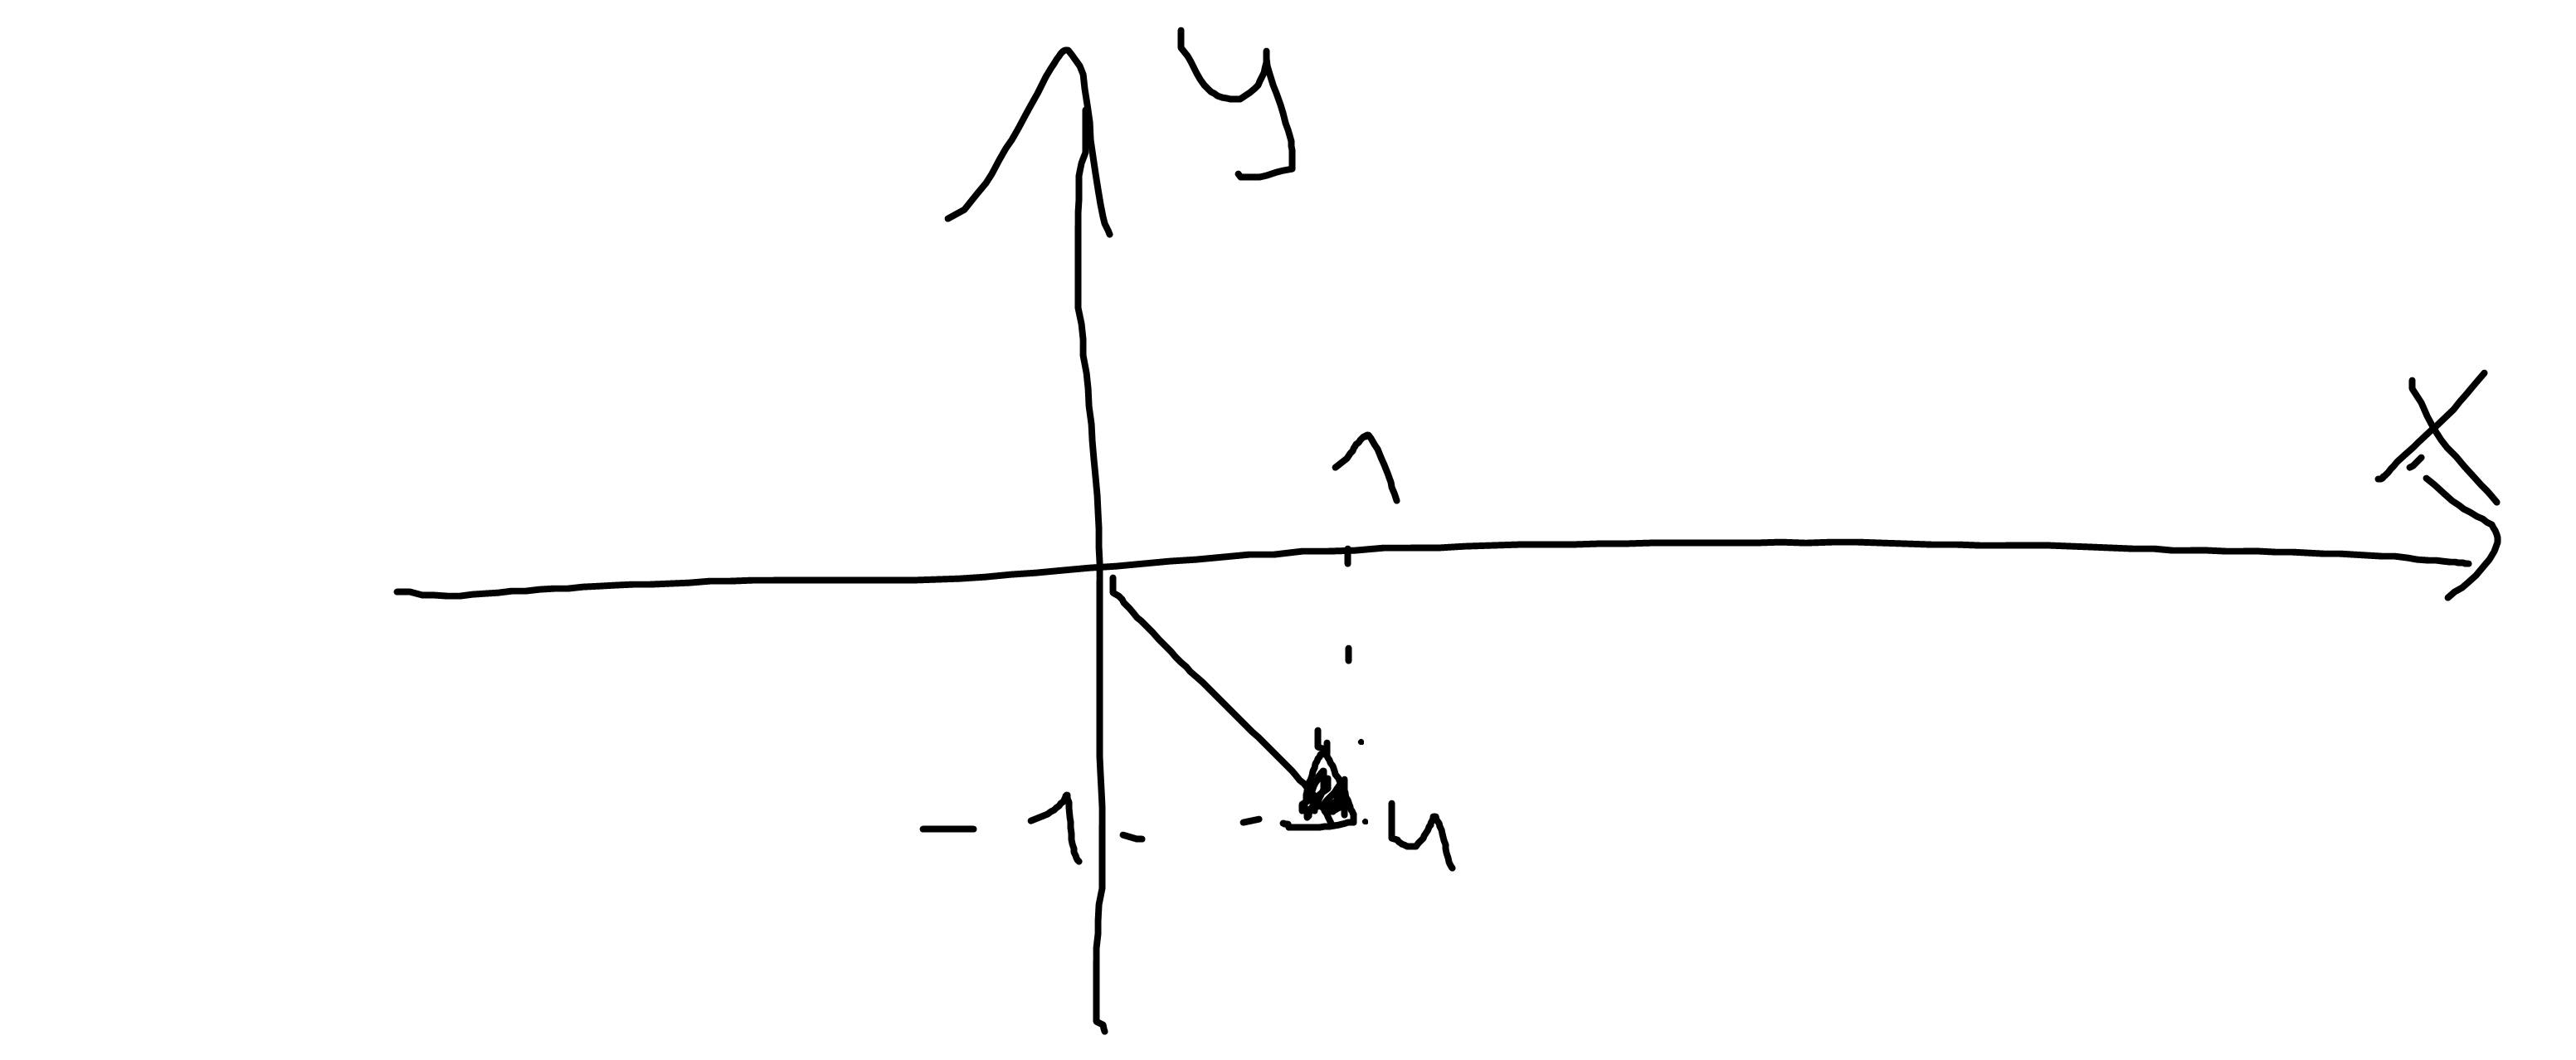
\includegraphics[height=3cm]{kepek/07.png}
			\caption{$l(t)=a+te,\quad  t\in\R$}
		\end{figure}
		\textit{Megoldás:} $a:=(1,1), e=\left(\frac{1}{2};\frac{\sqrt{3}}{2}\right)\in\R^2$
		\[ \Rightarrow\quad \norm{e}_2=\sqrt{\frac{1}{4}+\frac{3}{4}}=2\checkmark \]
		\[ \Rightarrow \quad F(t)=f(a+te)=f((1,1)+t\left(\frac{1}{2};\frac{\sqrt{3}}{2}\right))=f\left(1+\frac{t}{2};1+\frac{t\sqrt{3}}{2}\right)=\left(1+\frac{t}{2}\right)^2-\left(1+\frac{t}{2}\right)\left(1+\frac{t\sqrt{3}}{2}\right)+\left(1+\frac{t\sqrt{3}}{2}\right)^2\]
		\[\quad \Rightarrow\quad F\in D\quad \text{és} \]
		\[ F'(t)=2\cdot\left(1+\frac{t}{2}\right)\cdot\frac{1}{2}-\frac{1}{2}\left(1+\frac{t\sqrt{3}}{2}\right)-\left(1+\frac{t}{2}\right)\frac{\sqrt{}}{2}+2\left(1+\frac{t\sqrt{3}}{2}\right)\cdot\frac{\sqrt{3}}{2}\quad (t\in\R) \]
		\[\Rightarrow\quad \text{(def)}\quad \delta_ef(1,1)=F'(0)=2\cdot\frac{1}{2}-\frac{1}{2}-\frac{\sqrt{3}}{2}+2\cdot\frac{\sqrt{3}}{2}=\frac{1}{2}+\frac{\sqrt{3}}{2}=\frac{\sqrt{3}+1}{2}\in\R \]
		\begin{figure}[H]
			\centering
			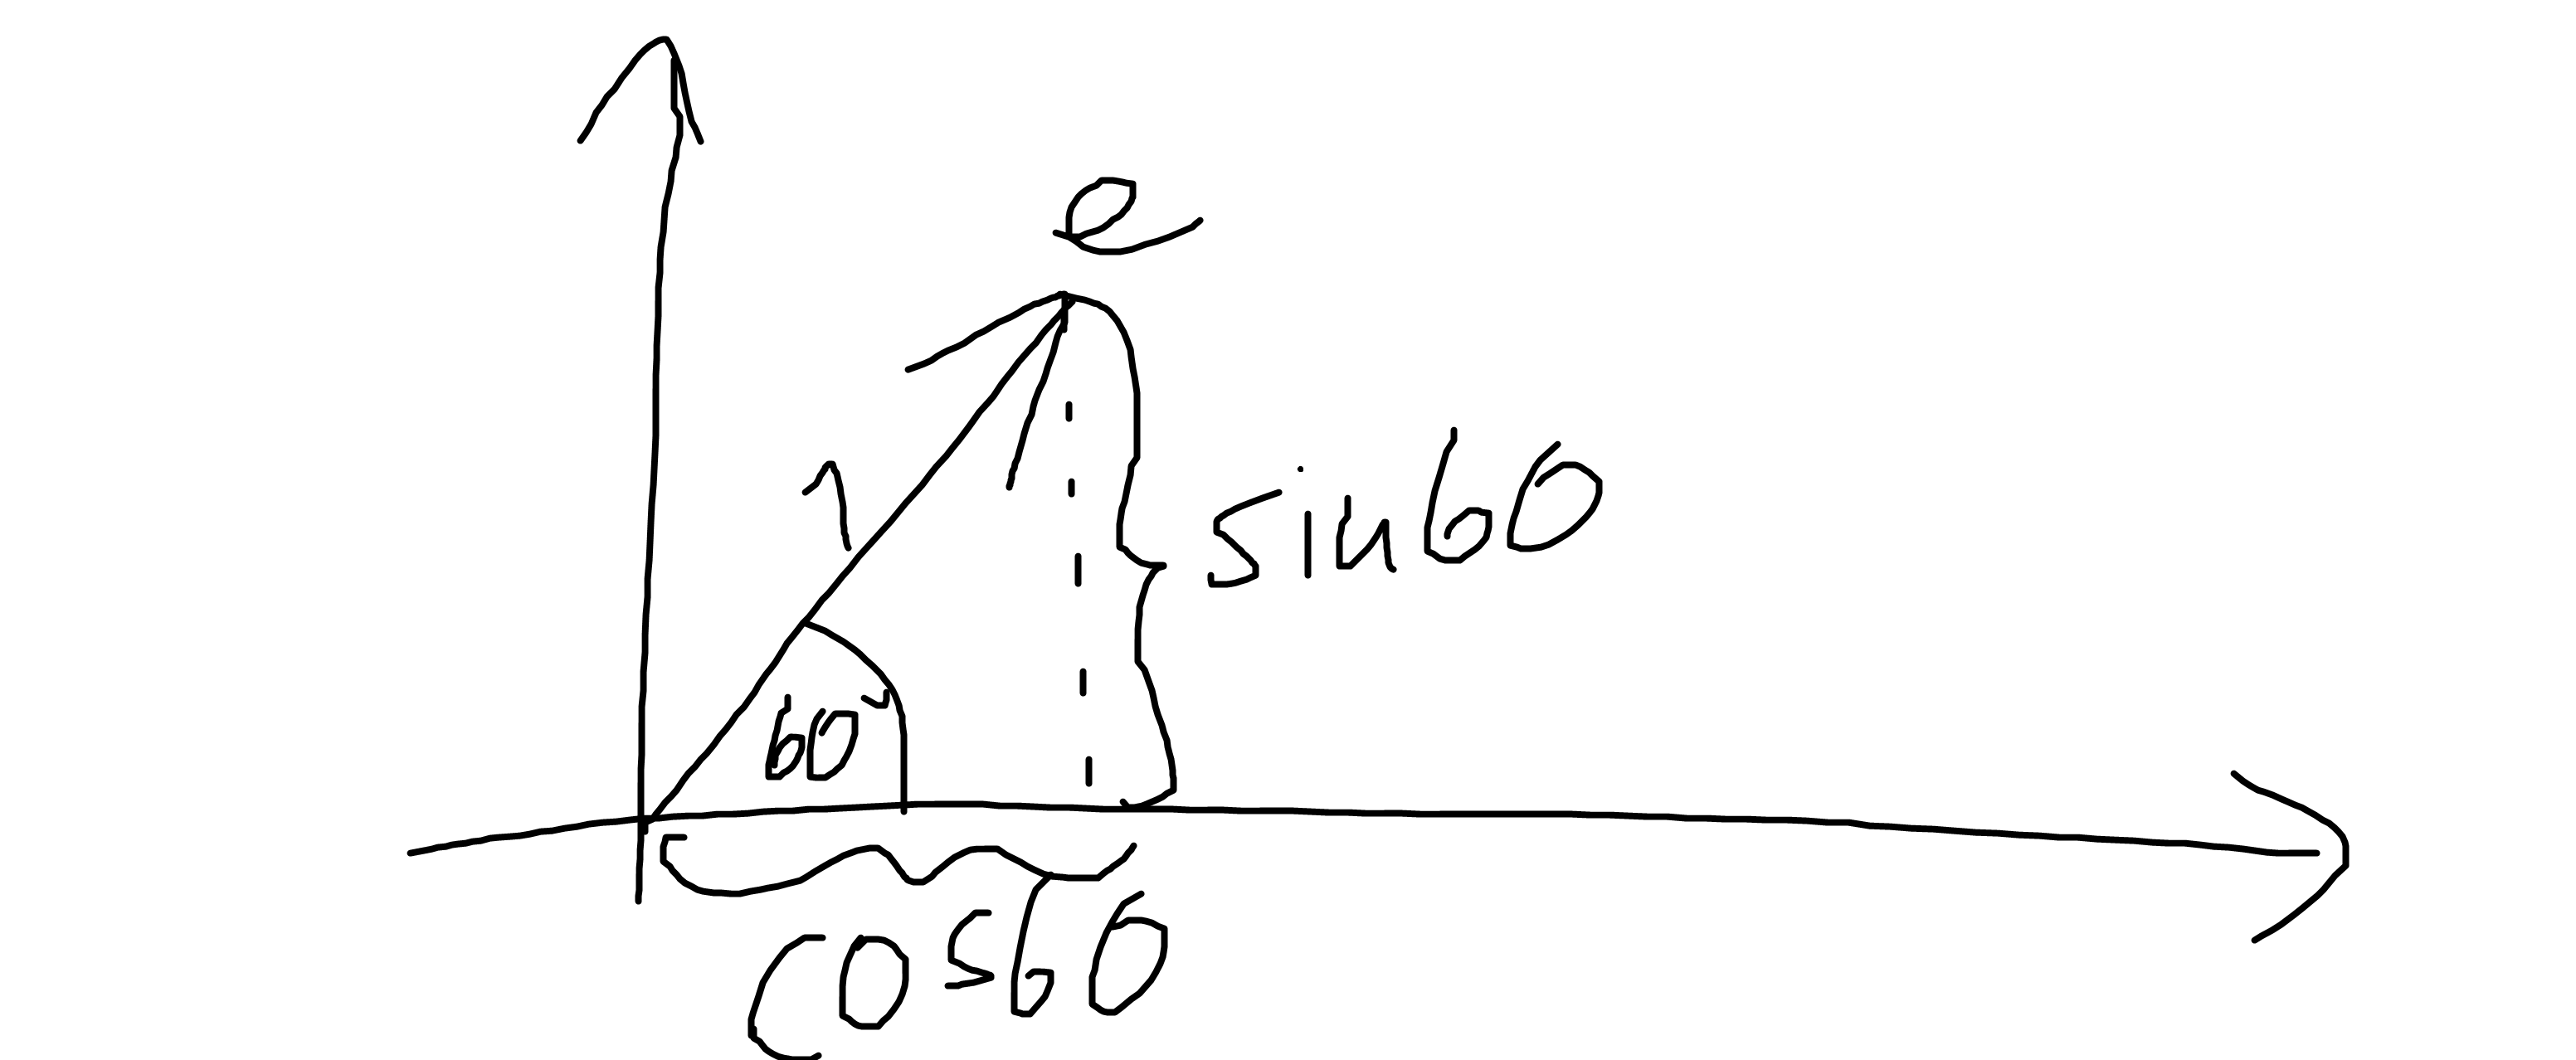
\includegraphics[height=3cm]{kepek/02.png}
			\caption{}
		\end{figure}
		
	\end{task}
	\begin{note}
		Ha nincs külön kijelentve, akkor kettes normával dolgozunk.
	\end{note}
	\begin{note}
		\begin{enumerate}
			\item Ha $f\in D\{a\}\quad \Rightarrow\quad \forall e\in\R^n,\quad \norm{e}=1$
			\[ \exists\delta_ef(a)=f'(a)\quad e=\langle f'(a),e\rangle \]
			Most: $\forall (x,y)\in\R^2$
			\begin{align*}
				\delta_1f(x,y)=2x-y\\
				\delta_2f(x,y)=-x+2y	
			\end{align*}
			Mivel $\exists\delta_1f, \delta_2f: \R^2\to\R$ és folytonosak:
			\[ \R^2\text{-en}\quad \Rightarrow\quad f\in D(\R^2) \]
			SPeciálisan:
			\[ f'(1,1)=(\delta_1f(1,1);\delta_2f(1,1))=(2\cdot1-1;-1+2\cdot1)=(1,1)=\grad f(1,1)\quad \Rightarrow\quad \exists\delta_ef(1,1)=\langle f'(1,1);e\rangle \]
			\[ =\langle(1,1),\left(\frac{1}{2};\frac{\sqrt{3}}{2}\right)=1\cdot\frac{1}{2}+1\cdot\frac{\sqrt{3}}{2}=\frac{\sqrt{3}+1}{2} \]
			\item Legyen $e:=(\cos\alpha; \sin\alpha)\quad \alpha\in[0;2\pi]$
			\[ \Rightarrow\quad \exists\delta_ef(1,1)=\langle f'(1,1);e\rangle\quad \overset{\norm{e}_2}{=}\quad \langle(1,1);(\cos\alpha,\sin\alpha)\rangle=\sin\alpha+\cos\alpha=:g(\alpha)\quad \Rightarrow \]
			$g'(\alpha)=\cos\alpha-\sin\alpha=0\quad \Leftrightarrow\quad \tg\alpha=0$
			\begin{figure}[H]
				\centering
				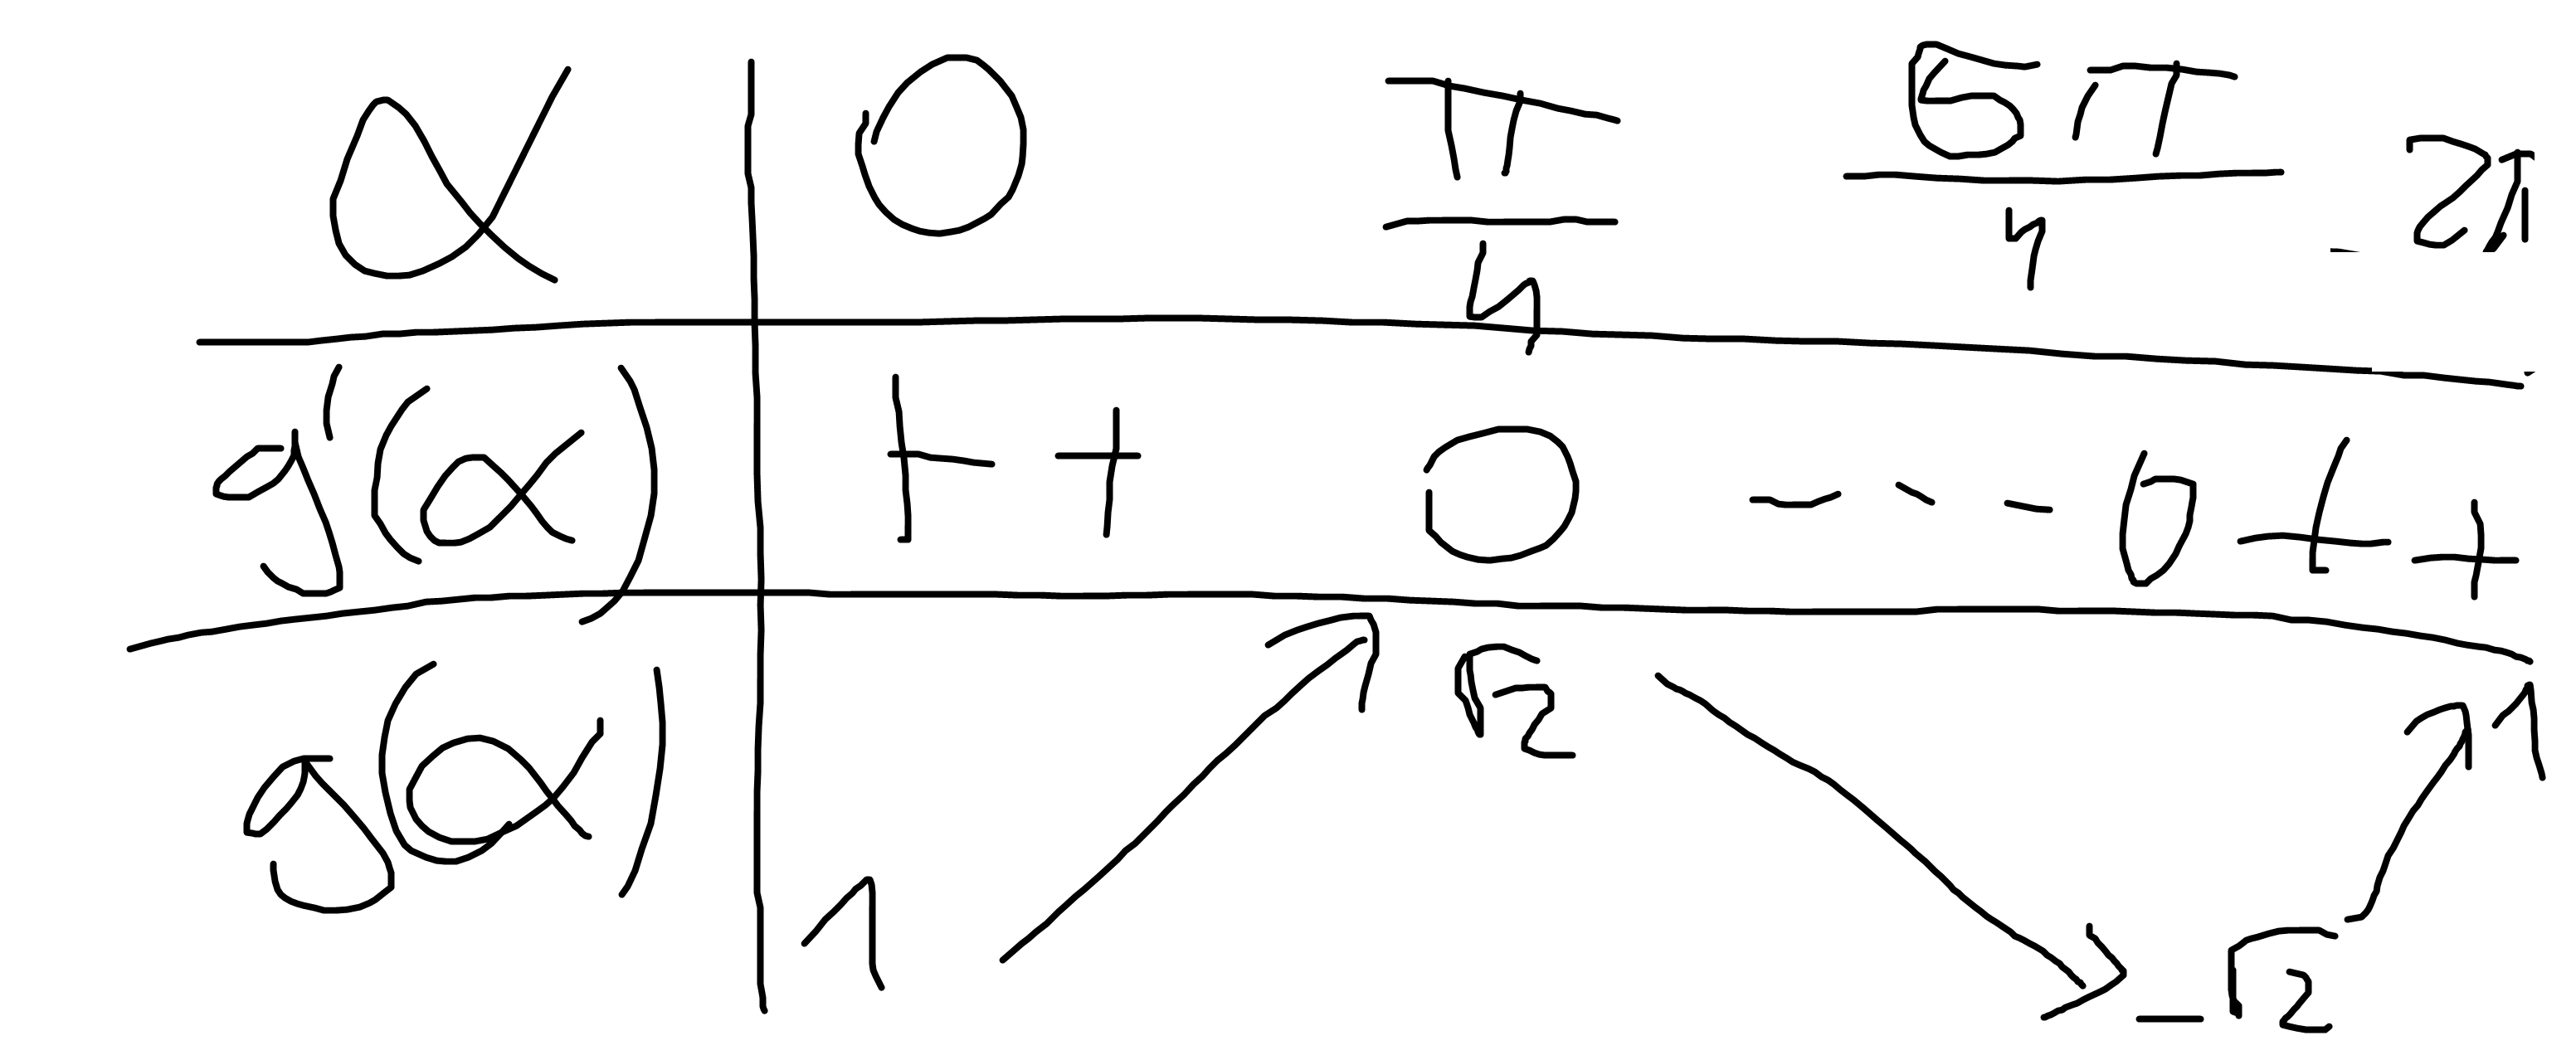
\includegraphics[height=3cm]{kepek/03.png}
				\caption{}
			\end{figure}
			\begin{figure}[H]
				\centering
				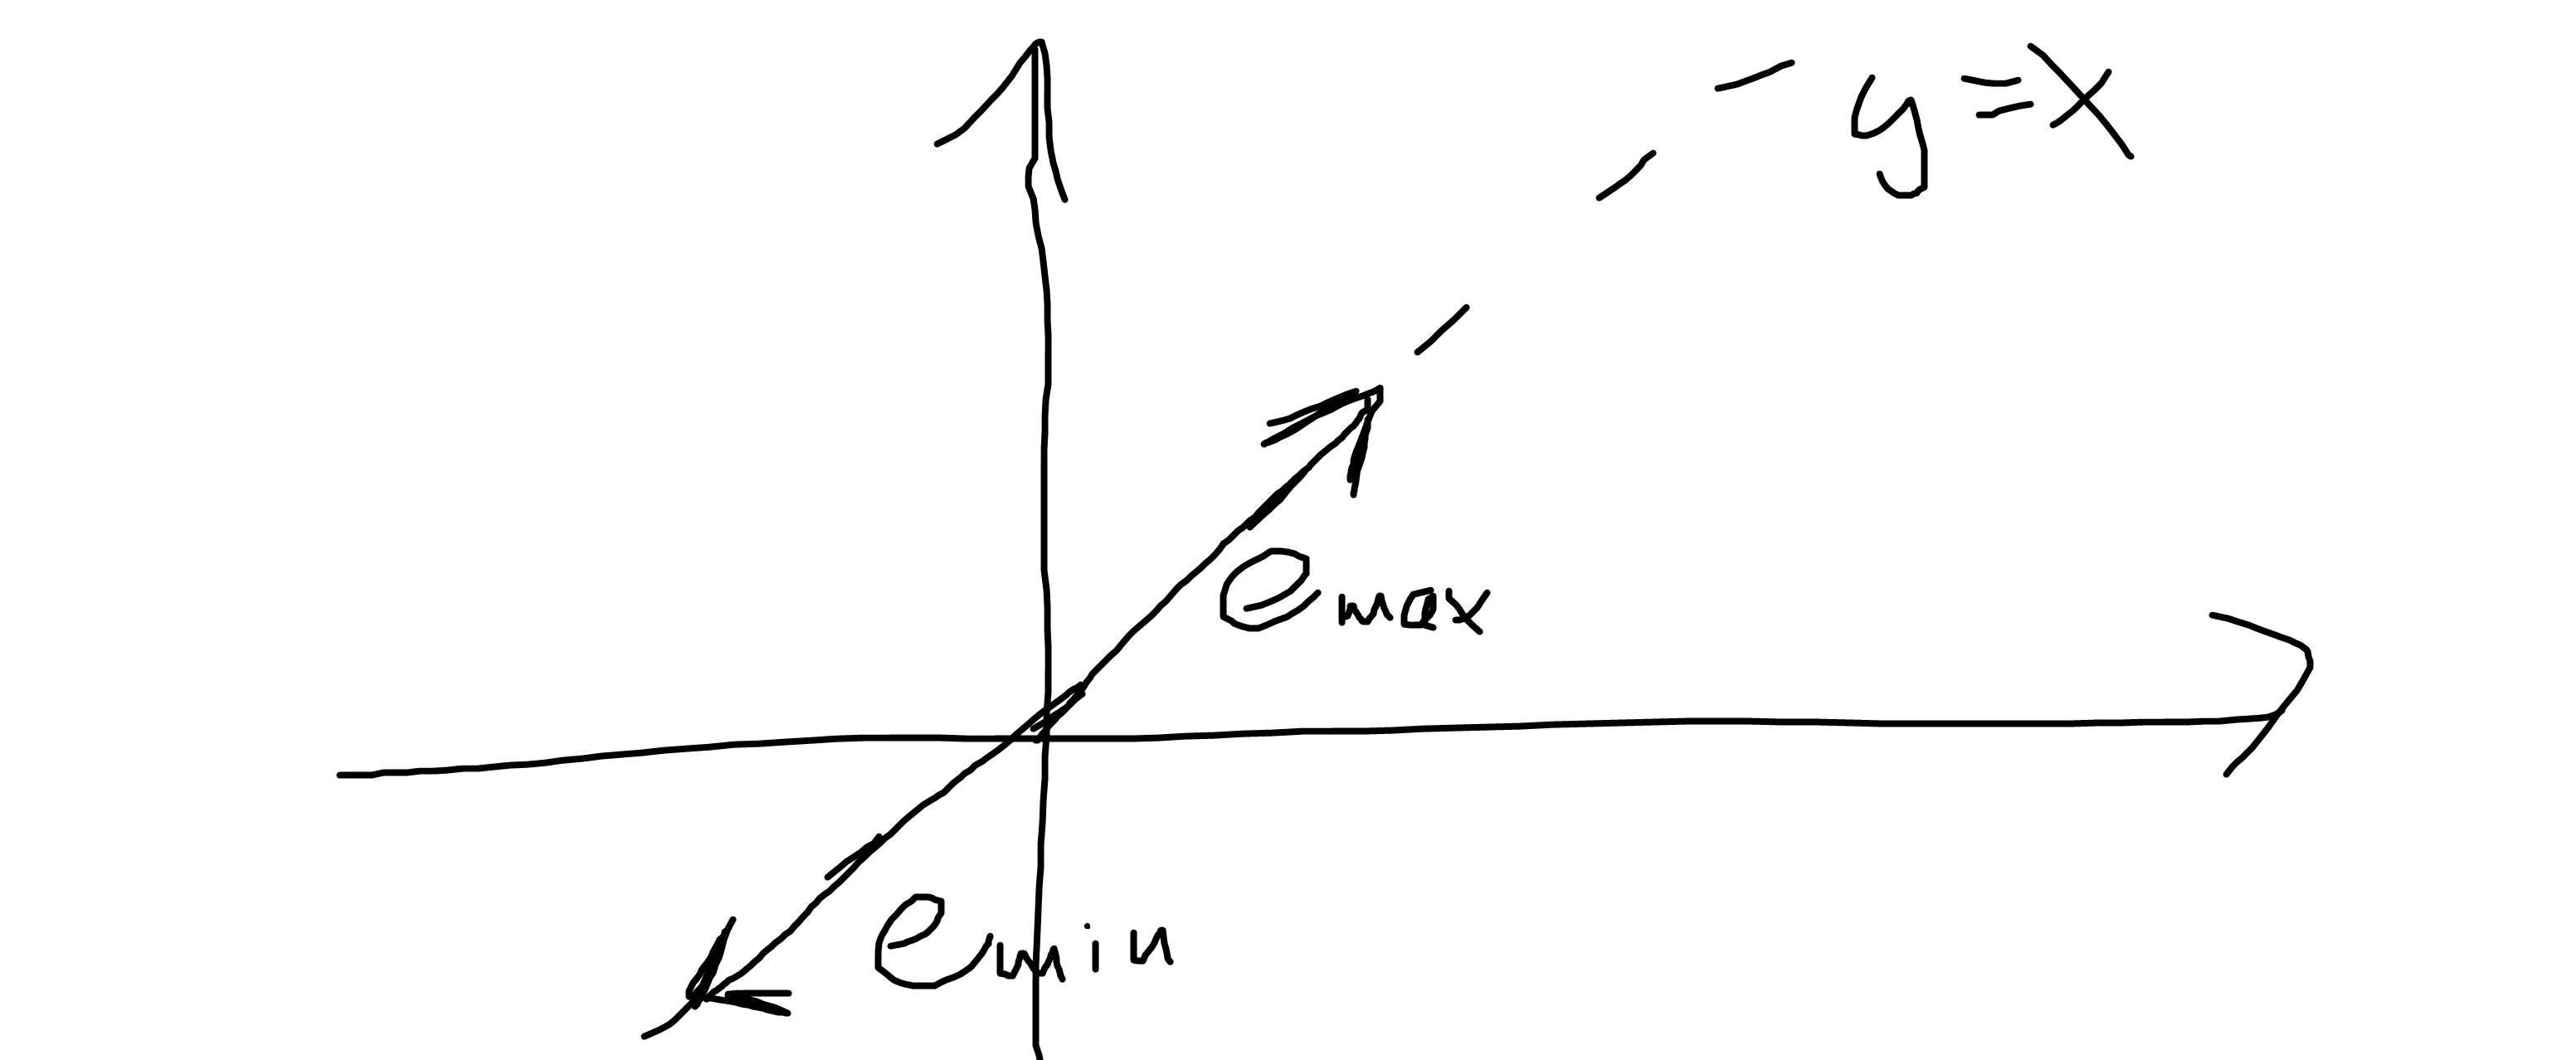
\includegraphics[height=3cm]{kepek/04.png}
				\caption{$e_{\min}= \left(-\frac{\sqrt{2}}{2};-\frac{\sqrt{2}}{2}\right),\quad e_{\max}= \left(\frac{\sqrt{2}}{2};\frac{\sqrt{2}}{2}\right)$}
			\end{figure}
			Véletlen, higy a max grádiens irányú? hf.
		\end{enumerate}
	\end{note}
	\begin{note}
		Legyen
		\[ f(x,y):=\begin{cases}
			1\quad (x,y)\in A\cup B\cup C\\
			0\quad \text{különben}
		\end{cases} \]
		\begin{figure}[H]
			\centering
			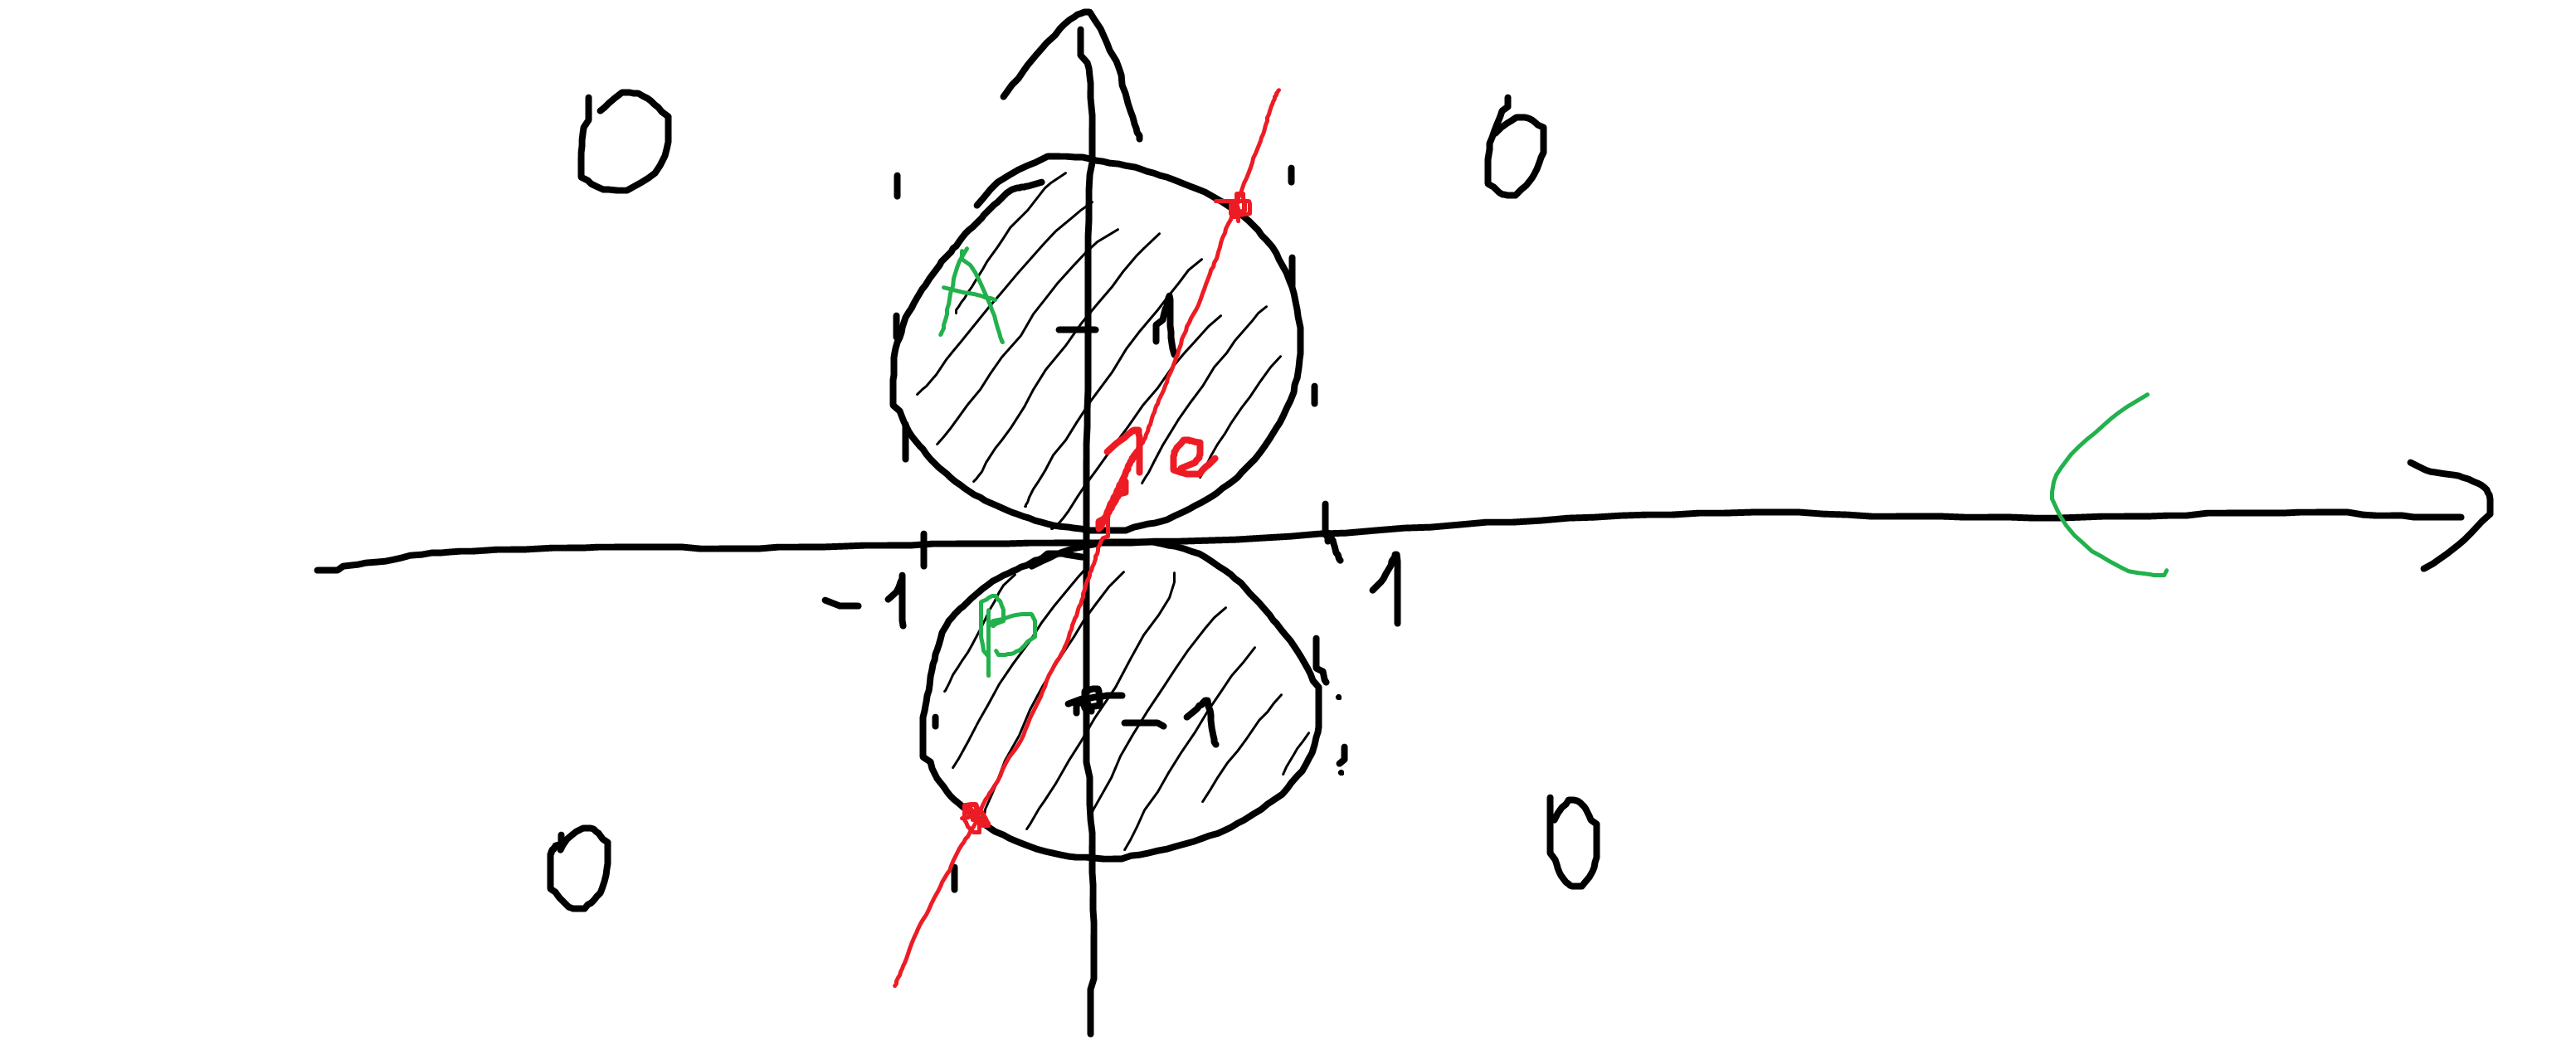
\includegraphics[height=3cm]{kepek/05.png}
			\caption{}
		\end{figure}
		$e$ fix.
		\begin{figure}[H]
			\centering
			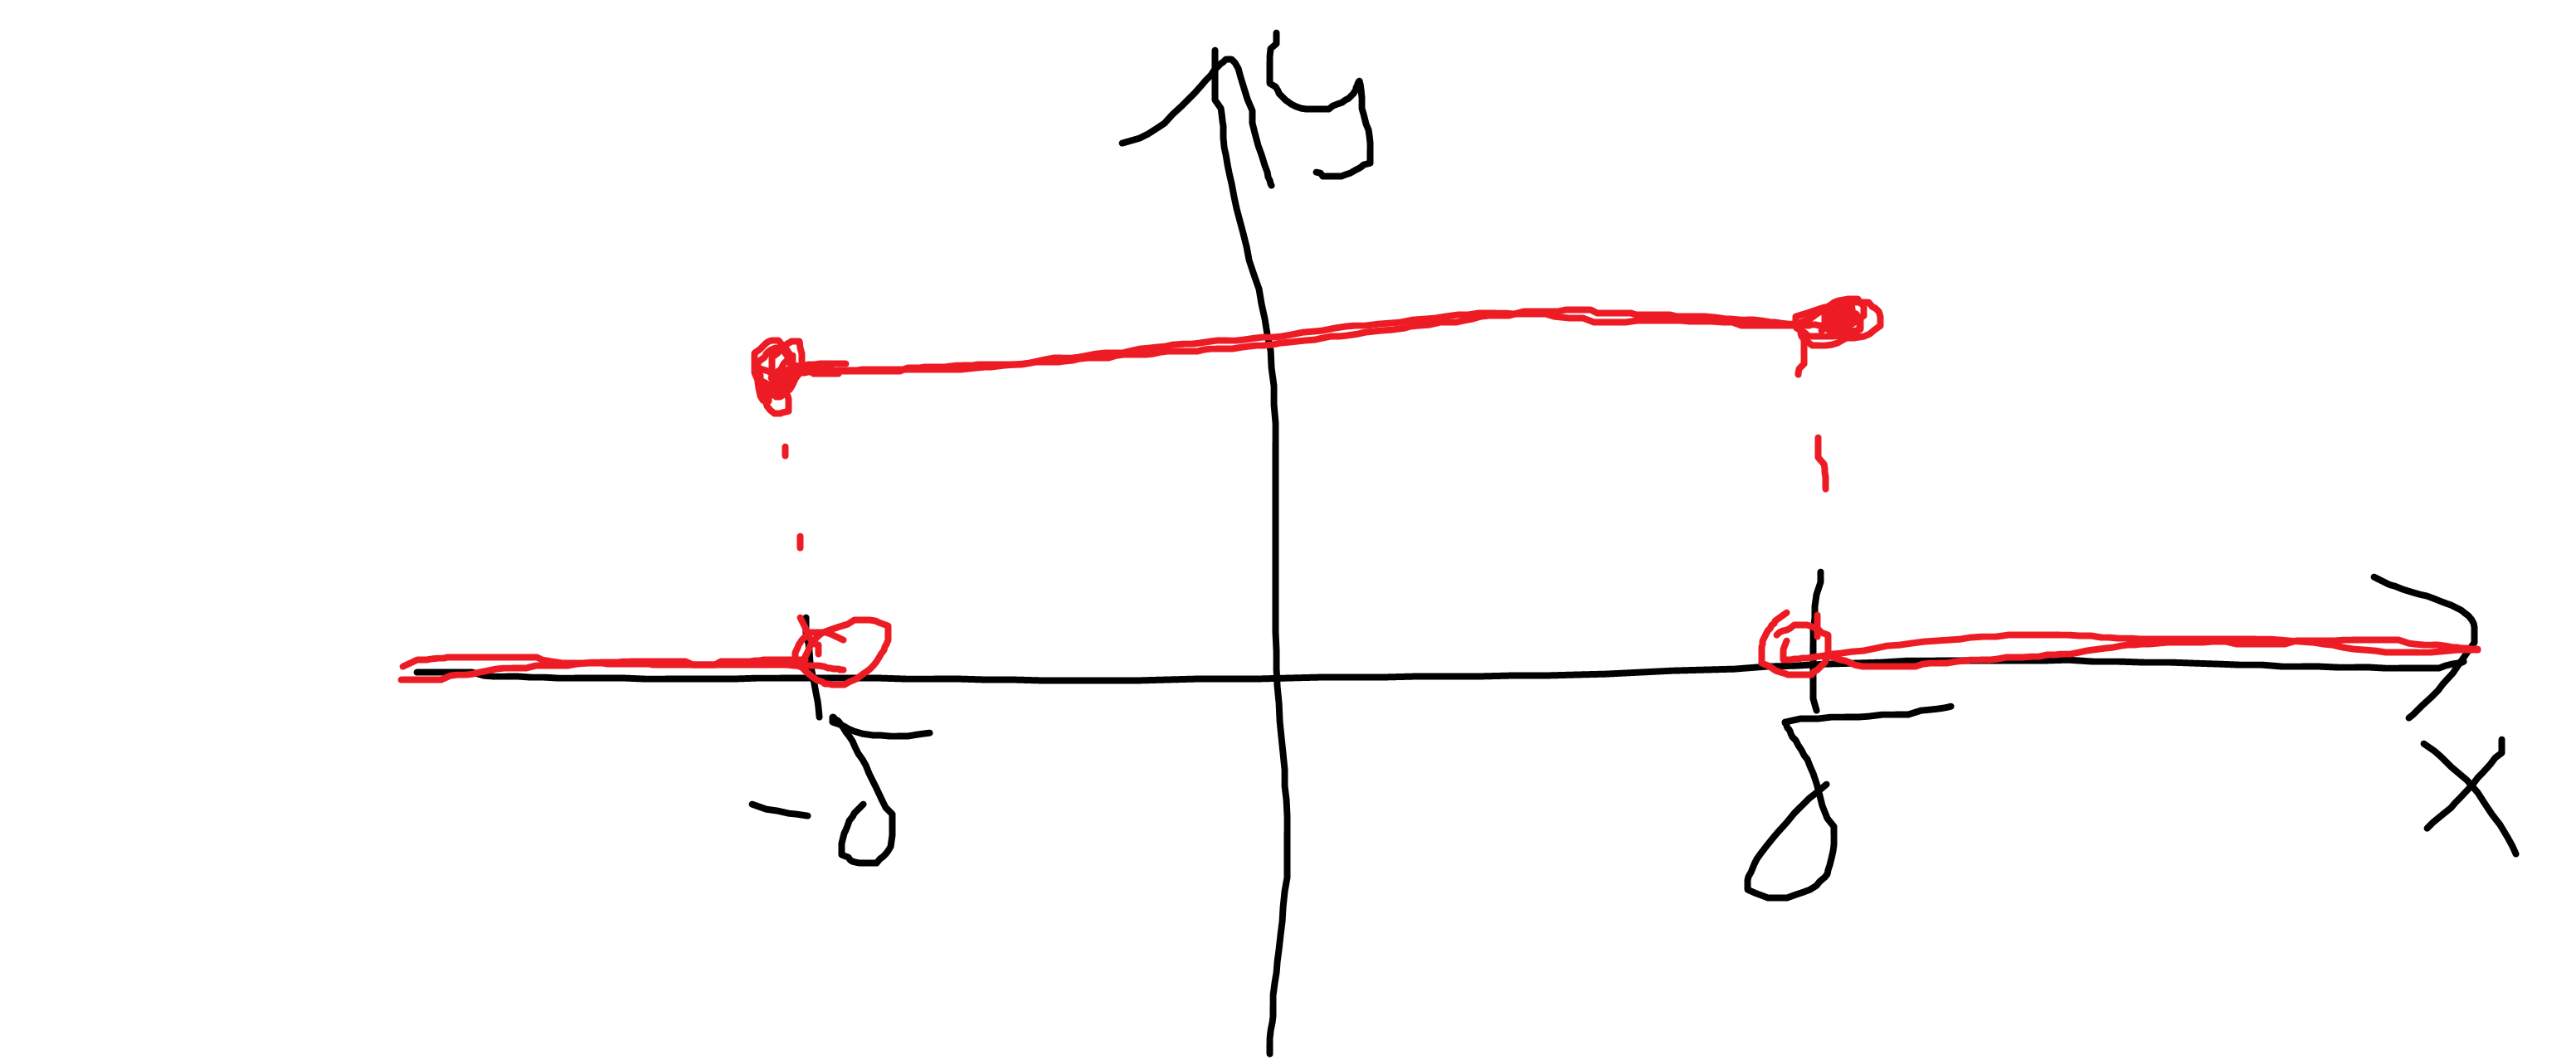
\includegraphics[height=3cm]{kepek/06.png}
			\caption{}
		\end{figure}
		\[ \Rightarrow\quad \exists\delta_ef(0,0)=0\quad (\forall e\in\R^2,\quad \norm{e}=1) \]
		De:
		\[ f\notin C\{(0,0)\} \quad \text{ui.}\quad \nexists\lim_{(0,0)}f\quad \Rightarrow\quad f\notin D(0,0) \]
	\end{note}
	\begin{center}
		\textit{,,Itt áll Gizi a Himalája tetején. Azt kérdezzük Gizitől, hogy indulj el, hogy a lehető legmeredekebb pályán menjél?''}
		
		/Filipp/
	\end{center}
	\begin{task}
		\[ f(x,y)=e^x\cdot y+x\cos y\quad ((x,y)\in\R^2) \]
		$a:=(0,1);\quad u:=(1,-\sqrt{3})\quad \Rightarrow\quad \delta_ef(a)=?\quad \text{ahol}\quad e$ az $a$ irányú egységvektor (kettes normával)
		
		Egyes normával hf.
		
		\textit{Megoldás (2es norma:)} 
		%TODO 07
		\[ e:=\frac{u}{\norm{u}_2} \]
		Ha más normában szmolnánk, ahhol más norma szerint kell ozstnai is.
		\[ e=\frac{(1,-\sqrt{3})}{\norm{1,-\sqrt{3}}_2}=\frac{(1,-\sqrt{3})}{ \sqrt{1^2+3}}=\left(\frac{1}{2},-\frac{\sqrt{3}}{2}\right) \]
		\begin{align*}
			\delta_1f(x,y)=&ye^x+\cos y\\
			\delta_2f(x,y)=&e^x-x\sin y
		\end{align*}
		$((x,y)\in\R^2)$, és $\delta_1f\delta_2f:\R^2\to\R$ folytonosak
		\[ f\in D(\R^2)\quad \text{spec.}\quad f\in D\{(0,1)\}\quad \text{és}\quad \Rightarrow\quad \exists\delta_ef(0,1)=\langle f'(0,1);e\rangle=\]\[\langle \delta_1f(0,1),\delta_2f(0,1);\left(\frac{1}{2},-\frac{\sqrt{3}}{2}\right)\rangle=\frac{1}{2}(1+\cos 1)-\frac{\sqrt{3}}{2}=\frac{1-\sqrt{3}-\cos1}{2} \]
	\end{task}
	\begin{task}$f:\R^2\to\R$ úgy, hogy: \quad ($\frown(x,y)\in\R^2)$
		\[ \begin{cases}
			\delta_1f(x,y)=x^2y\\
			\delta_2f(x,y)=1+\frac{x^3}{3}
		\end{cases} \]
		$f=?$
		
		\textit{Megoldás:} 
		\[f(x,y)=\int x^2y\,dx =y\cdot\int x^2\,dx=y\cdot\frac{x^3}{3}+c(y)\quad \text{ahol}\quad c\in\R\to\R,\quad c\in D \]
		Illetve:
		\[ \exists\delta_2f(x,y)=\delta_2\left(y\frac{x^3}{3}+c(y)\right)=\frac{x^3}{3}+x'(y)\quad \overset{\text{feltétel}}{=}\quad 1+\frac{x^3}{3}\quad \Rightarrow\quad c'(y)=1, \quad \text{azaz}\]
		\[\quad c(y)=\int1\,dy=y+c, \quad c\in\R \]
		Mivel most az $x$-es tagok kiesnek, így lesz eredmény. 
		Így a keresett függvények:
		\[ f(x,y)=y\frac{x^3}{3}+y+c\quad ((x,y)\in\R^2,\quad c\in\R) \]
	\end{task}
	\begin{note}
		Vajon csak $+c$ a derivált vége? A megoldás az hogy nem, bármilyen deriválható egyváltozós függvény mehet oda, mely $y$-tól függ.
	\end{note}
	\begin{note}
		\begin{enumerate}
			\item Legyen $g(x,y):=(x^2y;1+\frac{x^3}{3})\quad ((x,y)\in\R^2);\quad \Rightarrow\quad f:\R^2\to\R^2;$ azt kaptuk, hogy $\exists f:\R^2\to\R,\quad f\in D (?)$ és $f'(x,y)=(\delta_1f(x,y),\delta_2f(x,y))=g(x,y)$ vagy $f'=g$. EZt mondjuk, hogy $f$ a $g$ primitív függvénye.
		\end{enumerate}
	\end{note}
	\begin{task}
		\[ f(x,y):=\sqrt{|xy|}\quad ((x,y)\in\R^2) \]
		Bizonyítsuk be, hogy \begin{enumerate}
			\item $f\in C(0,0)$
			\item $\exists\delta_1f(0,0);\quad \delta_2f(0,0)=?$
			\item $f\notin D\{(0,0)\}$
		\end{enumerate}
		\begin{enumerate}
			\item 
			\[ \varepsilon>0\quad \text{fix.}\quad |f(x,y)-f(0,0)|=\sqrt{|x,y|}\quad \overset{\text{sz-m}}{\leq}\quad \frac{|x|+|y|}{2}=\frac{1}{2}\cdot\norm{(x,y)-(0,0)}_1<\varepsilon \]
			Ha $\norm{(x,y)-(0,0)}_1<2\varepsilon\quad \Rightarrow\quad \delta:=2\varepsilon$ jó a definícióhoz\quad $\Rightarrow\quad f\in\C\{(0,0)\}$
			\item \[\delta_1f(0,0)=g(0)=\lim_{x\to0}g(y)-g(0)=\lim_{x\to0}\frac{f(x,0)-f(0,0)}{x-0}=\lim_{x\to}\left(\frac{\sqrt{|x\cdot0}}{x}\right)=\lim_{x\to0}\frac{0}{x}=\lim_{x\to0}0=0 \]
			Illetve:
			\[ \delta_2f(0,0)=\lim_{y\to0}\frac{(0,y)-f(0,0)}{y-0}=\lim_{y\to0}\left(\frac{\sqrt{|0\cdot y|}}{y}\right)=0 \]
			AZaz, ha $f\in D\{(0,0)\}\quad \Rightarrow\quad f'(0,0)=(\delta_1f(0,0), \delta_2f(0,0))=(0,0)$
			A def. beli lim:
			\[ \lim_{(x,y)\to(0,0)}\frac{|f(x,y-f(0,0)-\delta_1f(0,0)-\delta_2f(0,0)}{\norm{x,y}_{\R^2}}=\lim_{(x,y)\to(0,0)}\frac{\sqrt{|xy|}}{|x|+|y|}\not=0 \]
			Ugyanis $x=y$ mentén:
			\[ \lim_{x\to0}\frac{\sqrt{|x|^2}}{2|x|}=\lim_{x\to0}\frac{|x|}{2|x|}=\frac{1}{2}\not=0\quad \Rightarrow\quad f\notin D\{(0,0)\} \]
		\end{enumerate}
	\end{task}
\end{document}